\chapter{Sistemas de recomendação}
\label{cap:sistemas_de_recomendacao}

% Introdução

% Falar sobre as mudança das coisas ligadas por "links" para por dados.

A web tem proporcionado diversas formas de interação, seja entre usuários ou entre sistemas e como resultado, tem-se uma grande quantidade de dados gerada. Os usuários que lidam com esses dados brutos certamente terão dificuldades em assimilar alguma informação útil e de seu interesse. Se faz necessário, portanto, um modo de processar tal montante de dados e extrair informações relevantes. Entre os possíveis métodos estão os mecanismos de busca, em relação à páginas web \cite{Brin1998}, e sistemas de recomendação, em relação a itens .
% Contextualizar com a Amazon, Netflix entre outros

% Os Sistemas de Recomendação surgem como potencial solução para esse problema. Um Sistema de Recomendação (SR) a partir de dados coletados sobre seus usuários na forma de preferências em certos conjuntos de itens, ou seja, produtos, eventos, ações entre outros e outras fontes de informação, provê aos usuários previsões e recomendações de itens de acordo c.

Sistemas de Recomendação (SRs) surgem como possível solução, com base na análise do perfil de cada usuário e, a partir deste, fornecer recomendações de itens que possam lhe interessar. Os itens recomendados podem ser filmes, livros, receitas, páginas web entre outros \cite{Bobadilla_2013}.  Deste modo, a tarefa de SRs é transformar os dados e preferências dos usuários em previsões de itens aos quais pode-se demonstrar interesse \cite{Lue2012}.

% Caracterizar
% Falar sobre os objetivos: previsão de avaliações, recomendação de itens.
% Definir item

%Falar sobre avaliações explícitas e implícitas
%(sobre os tipos de entradas que podem ser utilizadas

As informações de preferências de usuário, utilizadas como entrada por SRs, podem ser adquiridas de duas maneiras: explícita ou implicitamente. No primeiro caso, o usuário é indagado sobre suas preferências, já no segundo, as informações são extraídas de acordo com o comportamento do usuário e sem o questionamento direto \cite{Bobadilla_2013}. No entanto, informações adicionais podem ser utilizadas \cite{Jannach2010}. Deste modo, as fontes de informações utilizáveis são: avaliações de itens pelos usuários, conjunto de características específicas que o item deve possuir, além de detalhes sobre seu conteúdo. 

% Introduzir as abordagens e o que as diferencia
Os Sistemas de Recomendação são subdivididos em abordagens, filtragem colaborativa, baseada em conteúdo, baseada em conhecimento entre outras, às quais diferem na forma como geram sugestões e nas informações que utilizam para tal \cite{Jannach2010}. No entanto, décadas de pesquisa foram necessárias parar resultarem nas abordagens citadas.

\section{Histórico}

A web primordial ou Web 1.0 era estática, na qual a única perspectiva de interação era o consumo de conteúdo, ou seja, apenas leitura deste se fazia possível. Era, portanto, amplamente utilizada por organizações na divulgação de seus produtos e serviços \cite{Aghaei2012}. 

% Falar sobre a web 2.0, e interação do usuário.
A Web 2.0, por outro lado, agregou dinamicidade à Internet, desde a viabilização da interação entre usuários e possibilidade de inserção de conteúdo na rede por parte desses, a partir de blogs e redes sociais, por exemplo \cite{Nath2014}.

% Falar da web 3.0
Com a Web 3.0, se deu a transformação da Web de Documentos, presente nas versões anteriores, para a Web de Dados, onde os diversos conteúdos deixam de se relacionar por links e passam a ser por dados e, assim, podem ser utilizados não apenas por usuários, mas por máquinas.
%, às quais, usam a rede para acessar recursos externos entre outros.
 
%A web de documentos consiste em objetos, como websites, e as ligações entre eles, isto é, os \textit{links}, com foco no consumo de conteúdo por pessoas. A web de dados, entretanto, torna legível o conteúdo da web para as máquinas, priorizando estas em detrimento dos humanos a partir da representação e organização das dados formato organizado como o \textit{Resource Description Framework} (RDF) \cite{Aghaei2012}. Acrescentou-se, dessa forma, a possibilidade da comunicação entre dispositivos, além do aprimoramento do gerenciamento dos dados.

Já se discute a cerca da Web 4.0, apesar de, conceitualmente, não bem definida. Propõe-se que, no futuro, haveria uma simbiose entre os computadores e as pessoas e, como consequência, seria possível a construção de interfaces mais poderosas, entre elas, as controladas pela mente \cite{Aghaei2012}.

A ideia de fazer uso de todo o volume de dados gerados por muitos usuários, com a Web 2.0, para auxiliar na procura por conteúdos mais úteis e interessantes, já existia desde a década de 1990 \cite{Jannach2010}.

%    PARC Tapestry system
O primeiro sistema ao qual continha a ideia de recomendação de conteúdo, foi o PARC Tapestry System, que introduziu o conceito de filtragem colaborativa. Ademais, era um sistema experimental de e-mail, onde se objetivava categorizar o grande volume de mensagens eletrônicas recebidas em categorias de acordo com o interesse do usuário \cite{Goldberg1992}.
%    GroupLens - notícias
Alguns anos mais tarde, o \textit{GoodNews} foi desenvolvimento com o foco em notícias, onde cada artigo era avaliado de acordo com a média de avaliações dos usuários e os melhores eram recomendados. Dessa forma, o sistema não levava em conta gostos individuais e eliminava, assim, a necessidade de armazenamento de dados de usuários.
% Ringo system - filtragem colaborativa para músicas
Outro sistema desenvolvido, o Ringo, provia recomendações aos seus usuários a cerca de músicas. Inicialmente o utilizador fornecia avaliações  de aproximadamente 125 artistas e, de acordo com as respostas era feito uma avaliação do perfil.  A aplicação, então, passava a recomendar novos artistas e álbuns que o usuário poderia gostar \cite{Resnick1994}.

Com o passar dos anos, os Sistemas de Recomendação se expandiram para a área negócios, como o comércio eletrônico nos anos 2000 pela Internet. Ademais, se deu uma comercialização imediata e diversas companhias foram criadas como, \textit{Pattie Maes}, \textit{Net Perceptions}, entre outras. Por outro lado, não apenas pesquisadores apresentaram interesse, mas também profissionais da área de marketing. Por fim, desenvolveu-se novas abordagens baseadas em conceitos de inteligência artificial, recuperação de informação, mineração de dados, segurança, privacidade além de pesquisas em negócios e marketing \cite{Jannach2010}.


% Comercialização (...)
% Pesquisa (quais as pesquisar mais recentes
% Hoje (no que é usado, com qual finalidade);
% Definir item

\section{Filtragem Colaborativa (FC)} \label{sec:filtragem-colaborativa}
    
    Em diversas ocasiões do cotidiano as pessoas requisitam opiniões de outras a cerca de certos produtos ou serviços, seja filmes, restaurantes, equipamentos eletrônicos entre outros. A opinião do indivíduo, então, influencia na escolha do outro e o ajuda a tomar uma decisão sobre o problema. Por outro lado, um amigo recomenda a outro que assista um filme de ação em cartaz nos cinemas, sabendo que ainda não assistiu-o e que gosta de filmes do gênero. Esse indivíduo que recebeu a sugestão certamente levará em conta o conselho, assistirá o filme, provavelmente gostará dele e recomendará a um outro amigo que também não viu o filme.    
    Com base nesse contexto de recomendações entre indivíduos, tem-se o conceito de Filtragem Colaborativa (FC), no qual, a partir de um perfil de preferências de um certo indivíduo, obtido através de seu histórico, em conjunto com as opiniões de outros usuários semelhantes a ele, prevê quais os itens que tem a maior possibilidade de gostar ou de se interessar \cite{Jannach2010}.

    % Explicação do conceito: qual a ideia, objetivos, vantagens e desvantagens.
        % Características
        % Não precisa das características específicas dos itens.

    % Não precisa das características específicas dos itens.
    % processamento custoso
        % Escalabilidade comprometida
    % maior precisão

    %"Se usuários compartilham interesses, eles terão gostos parecidos no futuro".
    %Pegar recomendações apenas dos melhores match's.
    
    Os sistemas baseados em filtragem colaborativa se utilizam da matriz de avaliações de itens pelos usuários, como mostrado na Tabela \ref{tab:matriz-av-item-user}. Como saída, gera-se previsões de avaliações que usuários aplicariam para itens por eles não avaliados ou um conjunto de melhores itens para recomendação. Portanto, a partir do conjunto de dados da matriz é possível fazer uso de algoritmos que levem em conta as avaliações de todo o conjunto de usuários, para então definir qual é a avaliação plausível para um determinado item ou quais itens recomendar \cite{Bobadilla_2013}.
    
    \begin{table}[htb]
        
        \caption{Matriz de avaliações de itens por usuários}
        \label{tab:matriz-av-item-user}
        \begin{tabular}{@{}lcccccc@{}}
        \toprule
                  & Item 1 & Item 2 & Item 3 & Item 4 & Item 5 & Item 6 \\ \midrule
        Jack      & 5      & 4      & 2      & ?      & 5      & 1      \\
        Will      & 3      & 5      & 3      & 5      & 1      & 1      \\
        Elizabeth & 5      & 3      & 3      & 4      & 2      & 4      \\
        Hector    & 3      & 5      & 4      & 5      & 4      & 4      \\ \bottomrule
        \end{tabular}
        
        \footnotesize{Fonte: Autores}
    \end{table}
    
    Segundo \citeonline{Ricci2010}, os métodos de filtragem colaborativa podem ser agrupados em duas classes: os baseados em memória ou em vizinhança e os métodos baseados em modelo. A principal diferença entre as abordagens está no modo de uso da matriz de avaliações na geração de recomendações. 
    
    % Não precisa das características específicas dos itens.
    
    % Ideia
    % para cada fórmula, um exemplo
    % ex: quando mostrar o pearson, calcular a similaridade entre dois usuários.
        
    \subsection{Baseado em memória}
        % processamento custoso
        % Escalabilidade comprometida
        % maior precisão
        
        % Usam diretamente os dados da matriz
        Métodos de recomendação baseados em memória operam diretamente sobre a base de dados de avaliações de itens pelos usuários para geração de recomendações. Além disso, as recomendações estarão sempre atualizadas devido ao uso das mais recentes avaliações recebidas dos usuários \cite{Bobadilla_2013}. 
        
        % Rever
        %No entanto, para grandes bases de dados onde existem milhares de itens a serem avaliados e milhares de usuários, os métodos baseados em memória são lentos em termos de processamento, dificultando o seu uso em recomendações geradas em tempo real \cite{Mustafa2017}.
        
        Em geral, os sistemas produzem recomendações com base no conceito de vizinho mais próximos, onde o objetivo é encontrar semelhanças entre usuários ou entre itens com suporte nas diversas avaliações adquiridas pela base de dados \cite{Mustafa2017}. Por exemplo, se um usuário tem preferência em certos filmes de ficção científica e existe um outro que também tem algum gosto pelo gênero, ambos poderão ser classificados como vizinhos próximos. Em casos como esse, o grau de semelhança é obtido a partir de cálculos de similaridade.
        
        \subsubsection{Medidas de Similaridade} \label{sssec:similaridade}
        
        % Definição
        A similaridade entre usuários, itens, etc., podem ser obtidas a partir da matriz de avaliações dos usuários em relação ao itens. Os diversos algoritmos operam sobre as linhas ou colunas da tabela para encontrar um valor numérico que caracterize o grau de afinidade entre os objetos da comparação \cite{Aggarwal2016}. Além disso, uma abordagem geométrica pode ser utilizada para aprimorar a observação do comportamento desses algoritmos \cite{Jones1987}.
        
        % \subsubsection{Correlação de Pearson}
        O grau de semelhança entre dois usuários pode ser mensurado a partir de sua correlação, na qual estima a relação linear entre ambos. Dentre os diversos métodos, a correlação de \textit{Pearson} avalia vetores de mesma dimensão \cite{Ricci2010}. Considerando, um conjunto de produtos $P=\{p_1, p_2, ..., p_n\}$, um conjunto de usuários $U = \{u_1, u_2, ..., u_m\}$ e uma matriz de avaliações $R=\{r_{1,1}, r_{1,2}, ..., r_{n, m}\}$ desses produtos em função dos usuários, com dimensão  $n\times m$, tem-se a Equação \ref{eq:correlacao-pearson} que descreve a correlação de Pearson entre dois usuários $a$ e $b$.
             
        \begin{equation}
             % sim(a, b) =  \frac{\sum\limits_{i=1}^{n}(a_i-\bar{a})(b_i-\bar{b})}{\sqrt{\sum\limits_{k=1}^{n}(%a_k-\bar{a})^2}*\sqrt{\sum\limits_{j=1}^{n}(b_j-\bar{b})^2}} \label{eq:correlacao-pearson}
             sim(a, b) = \frac{\sum_{p\in P}(r_{a, p}-\bar{r_a})(r_{b, p}-\bar{r_b})}{\sqrt{\sum_{p\in P}(r_{a, p}-\bar{r_a})^2}\sqrt{\sum_{p\in P}(r_{b, p}-\bar{r_b})^2}}\label{eq:correlacao-pearson}
        \end{equation}
        
         Observa-se, inicialmente, a subtração de cada posição pelo valor médio das avaliações, o que reduz o efeito negativo, no cálculo, das notas de um determinado usuários que, em sua maioria, são ou altas, ou baixas. Além disso, tem-se um produto interno como numerador e a multiplicação dos comprimentos dos vetores de avaliação de cada usuário como denominador. Como possíveis resultados, a correção de Pearson gera valores entre $-1$ a $1$, onde o primeiro indica correlação negativa perfeita, ou seja, usuários com preferências opostas, e o segundo demonstra correlação positiva perfeita, implicando em gostos equivalentes entre os usuários \cite{Jannach2010}.
        
        %Pearson: É melhor entre outras técnicas para comparar usuários
        
        Como exemplo, considerando a Tabela \ref{tab:matriz-av-item-user}, deseja-se encontrar a similaridade entre os usuários Will e Elizabeth a partir de suas respectivas avaliações para os seis (6) itens e a correlação de Pearson. Fazendo uso da Equação \ref{eq:correlacao-pearson}, tem-se o seguinte cálculo:
        
        \begin{eqnarray}
            sim(W, E) &=& \text{\footnotesize   $\frac{(3-3)(5-3,5)+(5-3)(3-3,5)+...}{\sqrt{(3-3)^2+(5-3)^2+...}\sqrt{(5-3,5)^2+(3-3,5)^2+...}} $} \nonumber \\
            sim(W, E) &=& 0,21 \nonumber
        \end{eqnarray}
    
        Os usuários Will e Elizabeth têm portanto uma similaridade medida pela correlação de Pearson de $0,21$ indicando que ambos têm alguma semelhança entre suas preferências.
    
        %##########    Cosseno    ###################
        Em relação a similaridade de itens, o método do \textit{cosseno} é considerado o padrão. Como base para o seu cálculo, se faz uso das avaliações dadas por todos os usuários a cada item, ou seja, as colunas da matriz de avaliação são utilizadas. No entanto, o método do cosseno não leva em conta o perfil de cada usuário ao considerar apenas a avaliação dada ao item em questão\cite{Jannach2010}.
        
        A Equação \ref{eq:sim-cosseno} define o cálculo de similaridade pelo método do cosseno onde, calcula-se o produto interno entre os vetores de avaliações dos itens, como numerador e a multiplicação dos comprimentos de cada um como denominador.         
        
        %cosseno: É melhor que Pearson para comparar itens.
        %Jones
        \begin{equation} 
            sim(a, b) = \frac{\sum_{u\in U}(r_{u, a})(r_{u, b})}{\sqrt{\sum_{u\in U}(r_{u, a})^2}\sqrt{\sum_{u\in U}(r_{u, b})^2}} \label{eq:sim-cosseno}
        \end{equation}    
    
        Em outras palavras, para cada usuário $u$ pertencente ao conjunto de usuário $U$, é calculada a multiplicação das suas avaliações para cada item e somada aos demais resultados da operação e, por fim, calcula-se o módulo de cada vetor. Um outra interpretação para o cálculo é considerar como sendo o produto interno entre os vetores de avaliação normalizados \cite{Jones1987}. Assim, com a divisão pelo comprimento, os possíveis resultados permanecem entre $0$ e $1$ \cite{Jannach2010}, sendo que geometricamente, esses resultados podem ser avaliados como ângulos. As avaliações de um item podem ser consideradas componentes de um vetor que representa o objeto. Inserindo, então, os vetores num plano será formado um ângulo $\theta$ no qual, no contexto das avaliações de itens é obtido partir do arco cosseno do resultado da similaridade. Quanto mais próximo, esse ângulo estiver de zero grau ($0^o$), maior será a semelhança entre os itens.
        
        Como exemplo, pretende-se encontrar o grau de similaridade entre Item 2 e Item 5 da Tabela \ref{tab:matriz-av-item-user}. Para tanto, considera-se as respectivas colunas de avaliações que usuários forneceram à cada um e a Equação \ref{eq:sim-cosseno}. Por fim, tem-se o seguinte cálculo:
        
        \begin{eqnarray}
            sim(2, 5) &=& \frac{(4\cdot 5)+(5\cdot 1)+(3\cdot 2)+(5 \cdot 4)}{\sqrt{4^2+5^2+3^2+5^2}\sqrt{5^2+1^2+2^2+4^2}} \nonumber \\
            sim(2, 5) &=& 0,87 \nonumber
        \end{eqnarray}
        
        Os itens 2 e 5, portanto tem alta similaridade. Além disso, ao considerar a visão geométrica, têm-se um ângulo de $29,5^o$ formado entre os itens.
    
        %##########    Cosseno ajustado   ###################
        Como dito anteriormente, o método do cosseno não leva em conta o perfil de avaliações do usuário no cálculo da similaridade entre itens, no entanto, um método semelhante chamado \textit{cosseno ajustado}, corrige essa imperfeição. Primeiramente, define-se o cálculo pela Equação \ref{eq:sim-cosseno-ajustado}.
        
        \begin{equation}
             sim(a, b) = \frac{\sum_{u\in U}(r_{u, a}-\overline{r_u})(r_{u, b}-\overline{r_u})}{\sqrt{\sum_{u\in U}(r_{u, a}-\overline{r_u})^2}\sqrt{\sum_{u\in U}(r_{u, b}-\overline{r_u})^2}} \label{eq:sim-cosseno-ajustado}
        \end{equation}
        
        Observa-se, então, que o ajuste se refere à subtração da média das avaliações dadas pelo usuário $u$ a todos os itens. Assim, o efeito negativo causado pela média alta ou baixa de avaliações do usuário é reduzido, deslocando as avaliações para a média do usuário ao invés da média do item. Além disso, o intervalo de valores possíveis com o método do cosseno ajustado, diferentemente do cosseno, é de $-1$ a $1$ \cite{Jannach2010, Ricci2010}. Por outro lado, nota-se a semelhança do método do cosseno ajustado em relação à correlação de Pearson, descrita na Equação \ref{eq:correlacao-pearson}. No entanto, apesar de semelhantes, os contextos aos quais aplica-se cada método é diferente. A correlação de Pearson é utilizada para o cálculo de similaridade entre usuários, já o cosseno ajustado destina-se a encontrar a semelhança entre itens, apesar de ambas fazerem uso da média de avaliações de cada usuário.
        
        %
        \subsubsection{k Vizinhos Mais Próximos (kNN)}
            
            O kNN é um dos principais algoritmos para geração de recomendação e predições de avaliações \cite{Bobadilla_2013}, além de ter o objetivo geral de operar como classificador. Assim, dado um ponto em um espaço, o kNN encontrará os k pontos mais próximos com base em um conjunto de outros pontos pré-classificados e revelará à qual classe pertence. 
            
            Como exemplo, a \reffig{cap3_knn-no-class} traz dois conjuntos de pontos, azuis mais abaixo na imagem e vermelhos acima. Em meio a esses pontos à um outro, rosa, ao qual deseja-se saber à qual grupo pertence (independentemente de sua cor).             
            
            \begin{figure}[htb]
                \caption{Exemplo de grupos para classificação com o kNN}
                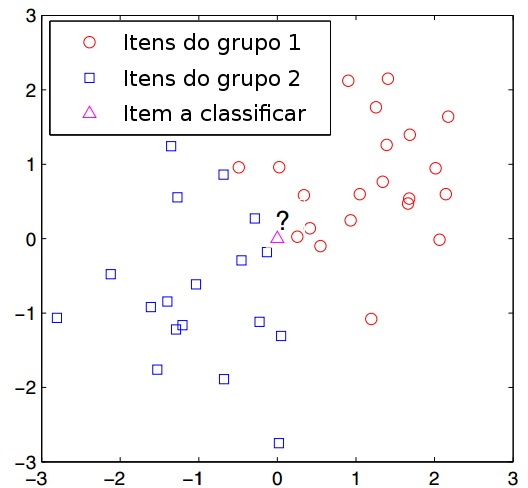
\includegraphics[width=0.55\textwidth]{cap3_knn-no-class}
                \label{fig:cap3_knn-no-class}
                
                {\footnotesize Fonte: Adaptado de \citeonline{Ricci2010}}
            \end{figure}
                        
            A partir de cálculos de similaridade o algoritmo encontrará os $k$ pontos mais próximos, onde tal valor varia de acordo o contexto da aplicação. \citeonline{Duda2000} sugerem um $k$  igual a raiz quadrada do total de pontos $n$, ou seja, $k$ é igual $\sqrt{n}$, no âmbito geral de classificadores, já no contexto de sistemas de recomendação, onde há bases com milhares de usuários, \citeonline{Jannach2010} afirma que $k$ entre $20$ a $50$ é uma boa estimativa. 
            
            Em um aspecto gráfico, $k$ pode ser interpretado como o número de pontos aos quais podem ser inseridos dentro de um círculo centrado no ponto que será classificado, como pode ser visualizado na \reffig{cap3_knn-class}. 
            
            \begin{figure}[htb]
                \caption{Exemplo de classificação com o kNN}
                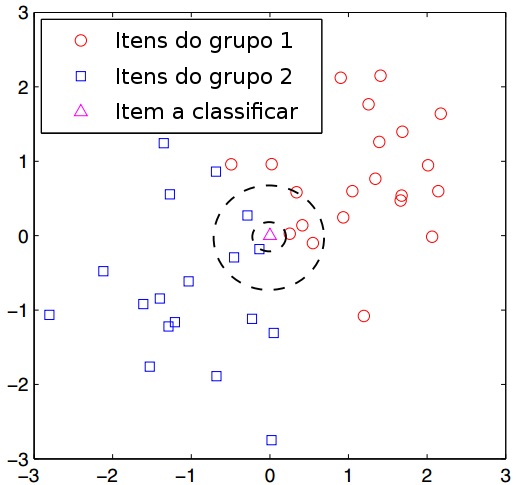
\includegraphics[width=0.55\textwidth]{cap3_knn-class}
                \label{fig:cap3_knn-class}
                
                {\footnotesize Fonte: Adaptado de \citeonline{Ricci2010}}
            \end{figure}            
            
            % CF baseado em kNN é simples e implementação direta
                 
            O algoritmo de $k$ vizinhos mais próximos opera em três etapas, sendo a primeira, a determinação dos vizinhos mais próximos do usuário $x$ conforme cálculos de similaridade. A seguir, previsões são computadas sobre as avaliações que $x$ daria a itens, aos quais, ainda não conhece, a partir de funções de agregação como, por exemplo, média e soma ponderada de notas de outros usuários ao item. Por fim, com base nas avaliações obtidas, os $m$ itens com melhores notas são recomendados ao usuário \cite{Bobadilla_2013}.
            
            
            % FC baseada em usuário
            O kNN pode ser aplicado nas duas categorias de filtragem colaborativa baseada em memória. A primeira delas é \textit{baseada em usuário}, onde as sugestões são fundamentadas em outros utilizadores com preferências semelhantes. Assim, os itens recomendados não foram comprados pelo usuário ou este não os conhece, no entanto os mais semelhantes o fizeram \cite{Ricci2010}. Contudo, a abordagem tem um custo elevado para processamento da matriz de avaliações e geração de recomendações, onde, a cada recomendação produzida, todos os cálculos são re-executados, ou seja, opera em modo \textit{online}.
            
            % FC baseada em item
            A segunda abordagem é \textit{baseada em item}, onde um item $i$ é avaliado e indicado com base nas notas que o usuário $u$ forneceu para itens similares aquele em questão. Itens são, então, similares se diversos usuários os avaliaram de maneira equivalente \cite{Ricci2010}. Ademais, o desempenho em termos de processamento, comparada à abordagem anterior, é superior, já que parte considerável do processamento pode ser feito \textit{offline} \cite{Jannach2010, Miranda2010}.
            
            %\subsubsection{FC baseada em usuário}  
            % mais custosa (online), toda vez que for recomendar, tem que calcular tudo de novo.
            % encontrar usuários semelhantes com 
            % Baseado em item
                        
            % \subsubsection{FC baseada em item}
            % compara os itens com base nas avaliações dos usuários. 
            % "Quem gosta desse item também costuma gostar deste".
            % Menos custos (offline)
    
    
    \subsection{Baseado em modelo}
    % processamento offline

        Sistemas de Recomendação baseados em modelo  não fazem uso direto da matriz de avaliações para geração de recomendação, contudo ela é utilizada para o aprendizado de um modelo, ao qual fará as recomendações \cite{Adomavicius2005}. Primeiramente, os dados de avaliações são processados internamente, ou seja, \textit{offline}, antes mesmo de  recomendações serem calculadas. Assim, no momento, em que se recomendar itens, apenas o modelo será necessário \cite{Jannach2010}. Entre as possíveis métodos para recomendação baseada em modelo tem a fatoração de matriz, métodos probabilísticos, redes neurais e baseados em regras de associação como se descreverá nas seções seguintes. 
        
        \subsubsection{Fatoração de matriz}
        
        Os modelos de fatoração de matriz levam em conta usuários e itens para explicar as avaliações dadas a partir de vetores de fatores resultantes da inferência dos padrões de notas \cite{Koren2009}. Tais fatores podem ser considerados características do item como, por exemplo, no contexto de livros, o autor, o gênero, no entanto, podem não ser interpretáveis, ou seja, não se consegue determinar a qual característica se refere. A partir disso, recomendações serão feitas quando usuários e item forem semelhantes em relação a esses fatores \cite{Jannach2010}. Por outro lado, o uso de avaliações explícitas pode não ser possível, devido à quantidade insuficiente de notas dadas por cada usuário. Apesar disso, o método permite o emprego de informações adicionais para obter as preferências de usuários. Avaliações implícitas obtidas a partir de seu comportamento além de históricos de compra, navegação e padrões de busca são utilizáveis nesse contexto \cite{Koren2009}. 
        
        
        %Entre as diversas técnicas existentes para encontrar os fatores latentes, há o método de Decomposição de Valor Singular (SVD), ao qual, afirma que uma matriz pode ser descomposta em um produto de outras três, como mostra a Equação \ref{eq:svd}, onde a $M$ é a matriz de avaliações $U$ e $V$ são os vetores singulares esquerdo e direito, respectivamente, e $\Sigma$ representa os valores singulares. E, como requisito, todas as matrizes devem ser quadradas \cite{Jannach2010}.
        
        % \begin{equation}
        %     M = U \Sigma V^T \label{eq:svd}
        % \end{equation}
                
        Entre as diversas técnicas existentes para encontrar os fatores latentes, há o método de Decomposição de Valor Singular (SVD). Neste modelo, cada item é ligado com um vetor $q_i$, no qual, os elementos indicam o quanto o item possui os fatores do vetor. Cada usuário é associado a um vetor $p_u$, que indica o grau de interesse do usuário nos itens que tem tais fatores altos ou baixos. Nesses casos, os valores que os fatores podem assumir estão entre $-1$ e $1$ .  A Equação \ref{eq:svd} demostra o cálculo para predição de avaliações do usuário $u$ ao item $i$ \cite{Ricci2010}.
        
        \begin{equation}
            \hat{r}_{ui} = \mu +b_u +b_i + q^T_ip_u  \label{eq:svd}
        \end{equation}
        
        Ao efetuar o produto $q^T_ip_u$ exprime-se o interesse do usuário nas propriedades do item. Os demais termos da Equação \ref{eq:svd} indicam a média global de avaliações de todos os itens ($\mu$) e os desvios, em relação a $\mu$, do usuário ($b_u$) e do item ($b_i$) \cite{Ricci2010}.
        
        Por fim, o SVD é capaz de gerar boas recomendações, entretanto é computacionalmente caro e deve ser executado \textit{offline}. Além disso, pode ser aplicado apenas em situações em que as informações de preferências não mudam com o tempo \cite{Bobadilla_2013}.
        
        \subsubsection{Métodos Probabilísticos}
        
        Os métodos probabilísticos procuram inferir a partir do uso de conceitos de estatística e probabilidade, as expectativas de eventos ocorrerem.  No contexto de SR, significa mensurar a possibilidade de um usuário avaliar um determinado produto com a nota determinada. Para tanto, pode se considerar a predição como um problema de classificação, onde se deseja colocar um objeto, entre diversas categorias, naquela que melhor se enquadra \cite{Jannach2010}.
                
        Entre os diversos métodos está o classificador de Bayes ao qual avalia a probabilidade de um evento ocorrer com base em outros eventos, ou seja, dados um conjunto de acontecimentos já decorridos no passado, qual a probabilidade de um determinado evento ocorrer no futuro. 
        Assim, o teorema de Bayes, descrito pela Equação \ref{eq:bayes}, pode ser usado pode ser utilizado para o cálculo da probabilidade para o evento \cite{Aggarwal2016}.
        
        \begin{equation}
            P(A \mid B) = \frac{P(B \mid A) \cdot P(A)}{P(B)} \label{eq:bayes}
        \end{equation}

        Considerando-se os eventos A e B, conforme Equação \ref{eq:bayes}, a expectativa de o evento A ocorrer no futuro sabendo que B transcorreu é determinada a partir da probabilidade do evento A ocorrer por si só ($P(A)$), do evento B, individualmente, ($P(B)$) e a probabilidade do evento B ocorrer em função de A ($P (B \mid A)$).
        
        No contexto de sistemas de recomendação o evento A, presente na Equação \ref{eq:bayes}, é visto como a probabilidade do usuário $u$ dar uma determinada nota $v_s$, dentre as possíveis notas, ao item $i$, tendo como base as avaliações já fornecidas por $u$. \cite{Aggarwal2016}
        
        \begin{equation}
              P(r_{ui} = v_s \mid r_u) = \frac{P(r_{ui}=v_s) \cdot P(r_u \mid r_{ui} = v_s)}{P(r_u)}
        \end{equation}
        
        O método probabilístico com o Teorema de Bayes apresenta algumas vantagens, entre elas, a compensação de pontos de ruídos nos dados de treinamento, não ter \textit{overfitting}, podendo assim aprender com modelos generalizados, além ser capaz de operar com um conjunto de dados pequeno \cite{Jannach2010}.
                
        \subsubsection{Redes Neurais}
        % o que são e onde pode usar
        Redes Neurais Artificais (RNAs) tentam retratar de forma matemática, o comportamento do cérebro biológico, ao qual é formado por células chamadas neurônios e suas diversas interconexões, onde, a cada uma das ligações, é atribuído um peso. Desse modo, a aprendizagem consiste em alterar, a partir de treinamento, os valores de cada peso a fim de se ter um comportamento específico para a rede. Além disso, a entrada e saída da rede é composta por um conjunto de neurônios que são ligados a parte externa da rede. \cite{Russell2009}. 
        
        A Figura \ref{fig:cap3_rna} mostra uma RNA chamada Percéptron de Múltiplas Camadas (MLP), onde os neurônios são representados por quadrados e elipses, e as conexões entre eles, por setas indicando os pesos a elas associados. A RNA mostrada tem duas entradas, representadas pelos neurônios um (1) e dois (2); dois neurônios, três (3) e quatro (4), na cada intermediária, também chamada oculta e, por fim, mais dois, cinco (5) e seis (6) na camada de saída.
        
        \begin{figure}[htb]        
            \caption{Rede Percéptron de Múltiplas Camadas}
            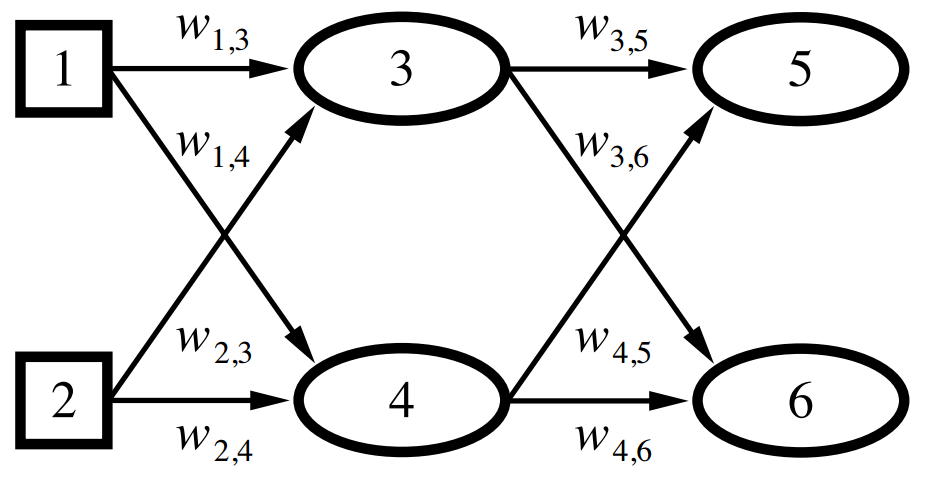
\includegraphics[width=0.6\textwidth]{cap3_rna}
            \label{fig:cap3_rna}
            
            \footnotesize{Fonte: \citeonline{Russell2009}}
        \end{figure}
        
        Redes neurais são capazes de aprender os padrões em dados de entrada e atuarem como classificadores. Entre as principais vantagens de RNA's de múltiplas camadas entre os demais classificadores é a capacidade de lidar com funções não-lineares, ou seja, a relação entre entradas e saídas é variável. \cite{Aggarwal2016}.
        
        No contexto de Sistemas de recomendação, redes neurais podem ser utilizadas para detectar padrões nas avaliações dadas pelos usuários aos diversos itens, e a partir disso, fazer predições de notas à itens que o usuário ainda não avaliou \cite{Ricci2010}. Assim, considerando uma matriz de avaliações de usuários para itens, como na Tabela \ref{tab:matriz-av-item-user}, a forma com a qual o usuário \textit{Jack} avaliaria o \textit{Item 4} pode ser determinada por RNA.
                  
        \subsubsection{Baseado em regras de associação}
        
        Há uma relação entre sistemas baseados em regras e os sistemas de recomendação baseados em regras, onde o primeiro foi proposto para a descoberta das relações entre transações. Assim, busca-se, por exemplo, descobrir qual a relação de compra de produtos entre as diversas transações, ou seja, se a aquisição de um item pode implicar na compra de outro \cite{Aggarwal2016}.  
        
        Recomendações são feitas para um usuário com base nas regras de associação que melhor se encaixam no seu histórico de transações.
        % Quem costuma comprar desse, compra desse outro também.
        Por fim, a partir de informações de relação de compras de produtos é possível aplicar promoções e mudança de layout de estabelecimentos \cite{Jannach2010}.
            
\section{Baseada em conteúdo}

    Sistemas de Recomendação baseados em conteúdo, aos quais têm como origens as pesquisas de filtragem de informação e recuperação de informação \cite{Cazella2010}, tentam recomendar itens ao usuário de acordo com as características de itens que ele gostou e das características do item em específico \cite{Ricci2010}. A recomendação será feita a partir da correspondência do perfil do usuário com as características dos itens. Assim, para esse tipo de sistema necessita-se apenas dos dados referentes aos itens, ou seja, sua descrição, e às preferências de usuário, isto é, seu perfil, não carecendo de uma grande comunidade de usuários para fazer recomendações. \cite{Jannach2010}. 

    \subsection{Descrição do item}
   
    Um item pode ser descrito em termo de seus atributos ou de seu conteúdo. No contexto de SR baseado em conteúdo essa definição pode ser obtida a partir de duas formas, sendo elas a explícita e implícita \cite{Jannach2010}. A forma explícita faz uso de características bens definidas dos itens. No caso de um livro, por exemplo, essas características são autor, gênero, preço, número de páginas entre outros. Em um sistema de recomendação essas informações devem ser inseridas manualmente para que possam ser utilizadas nos algoritmos. Por outro lado, a forma implícita faz uso de algoritmos que extraem informações dos itens. Além disso, essa abordagem é amplamente utilizada no contexto de recomendação de documentos textuais como, por exemplo, artigos científicos \cite{Garcia2013}.
    
    % Entre as principais formas de revelar as melhores palavras para representar o documento está a abordagem booleana, ao qual.
    
    Entre as diversas abordagens de representação de itens textuais está o modelo vetor de espaço baseado em palavras-chave. Nesse caso, busca-se representar um item por um conjunto de palavras melhor o descrevem \cite{Jannach2010}.
    
    Um padrão seguido para SR baseada em conteúdo para documentos textuais é usar o conteúdo em si do item para gerar recomendação e não os meta-dados, ou seja, as informações sobre o item. Entre as abordagens que aplicam esse conceito está a TF-IDF, onde os itens são representados como vetores de pesos, sendo cada posição correspondente a um termo com sua respectiva relevância. 
    %Contudo, é possível interpretar as posições como sendo características do item. 
    O TF-IDF é composto de um produto de dois pesos, o primeiro a Frequência do Termo (TF) e a Frequência Inversa do Documento (IDF), onde TF indica a frequência de cada termo no documento. No entanto, documentos maiores terão frequências maiores para as palavras e os menores o contrário, tornando injusta a medição por frequência absoluta. Por isso, é necessária uma normalização \cite{Jannach2010}. 
    
    A Equação \ref{eq:tf} apresenta o cálculo do TF, onde calcula-se a frequência normalizada de um termo $i$ em um item $j$ com base na frequência absoluta do termo no documento dividido pela número de ocorrências da palavra mais frequente entre no documento \cite{Jannach2010}.
     
    \begin{equation}
        \operatorname{TF}(i,j) = \frac{\operatorname{freq}(i,j)}{\operatorname{maxOutros}(i,j)} \label{eq:tf}
    \end{equation}
    
    Já o IDF tem por objetivo reduzir o impacto de palavras demasiadamente frequentes, ou seja, que são comuns em diversos documentos, como preposições e artigos. A Equação \ref{eq:idf} demonstra o cálculo do IDF para o termo $i$ de acordo com o número total de documentos recomendáveis $N$ e $\mathrm{n}(i)$, o número de documentos em que $i$ aparece \cite{Jannach2010}.
    
    \begin{equation}
        \operatorname{IDF}(i) = \log\left(\frac{N}{\operatorname{n}(i)}\right) \label{eq:idf}
    \end{equation}
        
    O cálculo de TF-IDF é, portanto, definido pela Equação \ref{eq:tf-idf}
    
    \begin{equation}
        \operatorname{TF-IDF}(i,j) = \operatorname{TF}(i, j)\cdot \operatorname{IDF}(i) \label{eq:tf-idf}
    \end{equation}

    
    Por fim, técnicas são necessárias para eliminar termos irrelevantes do documento. A primeira se refere a retirada de palavras de parada, como artigos e preposições. Outra técnica, lematização, consiste em substituir palavras semelhantes por sua palavra original, como ``ligado'', ``ligou'' e ``liga'' poderiam ser trocadas por ``ligar''. Outra maneira é reduzir o tamanho do vetor que representa o item, para as $n$ palavras que melhor o representam \cite{Jannach2010}.
    
     
    \subsection{Perfil de usuário}
    
    O perfil do usuário consiste num conjunto de características em que demonstrou-se, no passado, interesse por parte do indivíduo. Além disso, tal perfil pode ser adquirido de duas maneiras: explícita ou implicitamente. Na abordagem explícita, o usuário é diretamente indagado sobre seus gostos e preferências através de um conjunto de questionamentos elaborados pelo sistema e, fundamentando-se nas respostas, o perfil é traçado \cite{Adomavicius2005}.
    
    Na forma implícita, por outro lado, é utilizado o histórico do usuário para extrair suas preferências a partir de algoritmos de aprendizado de máquina ou \textit{machine learning}. Segundo \citeonline{Mitchell1997}, aprendizado de máquina consiste em permitir que um computador aprenda a executar um conjunto de tarefas a partir de um conjunto de dados de experiências prévias.
    Entre as técnicas de aprendizado de máquina aplicados a extração de perfil de usuário estão Árvores de Decisão, Redes Neurais, Feedback de Relevância além da computação evolucionária a partir algoritmos genéticos e, por fim,  métodos probabilísticos \cite{Ricci2010}.
   
    \subsection{Recomendação}
    
    Recomendações são feitas, no contexto de vetores de espaço, a partir da combinação dos vetores que descrevem os itens com o vetor que descreve as preferências de usuário. Assim, os itens com maiores semelhanças com o perfil do usuário são recomendados \cite{Aggarwal2016}.
    % No entanto, é possível também fazer recomendações a partir da comparação das características dos itens que o usuário tem preferência com as apresentadas nos itens aos quais se pretende recomendar. Isso se torna possível graças às medidas de similaridade, conforme visto na Seção \ref{sssec:similaridade}.

    % Falar sobre descrição do item 
    %     Explícita
    %         Características bem definidas (autor, afins)
    %     Implícita
    %         TF-IDF
    %             Documentos e itens
    % Perfil do usuário
    %     explícito
    %         baseado em regras
    %     implícito
            
    %             frequência
    %             binário
                
    %         a partir de histórico
    %         machine learning
            
    %         árvores de decisão
    %         Indução de regras
    %         kNN
    %             estruturado - distancia euclidiana
    %             não-estruturado - cosseno
    %         redes neurais
    %         AG
    %         Redes 
    % Recomendação
    %     Vetores
    %         Multiplicação de vetores: quanto maior melhor
        
\section{Baseada em conhecimento} 
    
Quando se trata de recomendar, nem sempre se terá à disposição uma base de dados com o histórico de interações de usuários. Além disso, mesmo com a existência de tal base,  os dados contidos podem não ser úteis quando trata-se de itens com longa duração como carros, casas, entre outros, onde a ocorrência de compras é muito baixa, em torno de anos \cite{Jannach2010}. Assim, as abordagens descritas anteriormente, ou seja, baseada em filtragem colaborativa e baseada em conteúdo, não são aplicáveis já que não há uma base de dados confiável para extrair informações e traçar um perfil para cada usuário  \cite{Ricci2010}. Por outro lado, há ocasiões em que o usuário esteja disposto a adquirir um produto que possua um conjunto de características específicas. 

Em meio às situações descritas, surge uma abordagem denominada recomendação baseada em conhecimento. Essa abordagem explora outros meios de informações, sendo elas informações sobre o usuário e sobre o item.
Assim, pode ser descrita como uma forma de se obter um conjunto de itens para recomendação aos quais satisfazem um conjunto de restrições definidas pelo usuário, podendo ser características, recursos, etc. \cite{Jannach2010}.

Segundo \citeonline{Ricci2010} e \citeonline{Aggarwal2016}, há dois tipos especí sendos eles, baseado em restrições e baseado em casos, que diferem de acordo com o modo utilizado para obter itens para indicação.

\subsection{Baseado em restrições}
    É mais rígido onde apenas itens com as características definidas pelas regras são escolhidos. Além disso, a tarefa de levantar um conjunto de itens que satisfaz as necessidades do consumidor é denotada como uma tarefa de recomendação \cite{Ricci2010}. Segundo \citeonline{Schreiber1999}, tarefa define, em termos de pares de entrada e saída, um objetivo de raciocínio. Assim, a tarefa de recomendação busca a partir de um conjunto de requisitos elencar um conjunto de itens que os satisfaz.
    
    %A tarefa é executada sobre uma base de conhecimento, ao qual contém regras que relacionam os requisitos do usuário com as características dos itens. Assim, a base é formada por dois conjuntos de variáveis, $V_C$ e $V_{PROD}$, e três conjuntos de restrições, $C_R$, $C_F$, $C_{PROD}$, $C_C$.
    %O primeiro conjunto de variáveis, $V_C$, tratá das propriedades do usuário, ou seja, a descrição possível dos requisitos de usuários como peso, tamanho etc. Já o outro conjunto de variáveis, $V_{PROD}$, descreve as propriedades de um dado item pode ter.
    
   % Por outro lado, em relação ao conjunto de restrições, o primeiro deles, $C_R$, restringe sistematicamente os possíveis valores das propriedades de usuários, como por exemplo, a propriedade ``tamanho'' deve ter o valor ``pequeno''.
    %O segundo conjunto, $C_F$, define condições de filtragem e define a relação entre o usuário e um produto. O terceiro conjunto, $C_{PROD}$ define os possíveis valores que as propriedades que o item pode ter como, por exemplo, a propriedade ``tamanho'' para um item, pode assumir os valores ``pequeno'', ``médio'', ``grande''. Por fim, o último conjunto, $C_C$ se refere às restrições que representam requisitos do usuário.
    
  %  Com base nos conjuntos de restrições e de variáveis, uma solução para o problema de satisfação de restrições consiste em instanciações das variáveis de tal forma que as restrições especificadas são atendidas. Para tanto, faz-se uso de algoritmos de satisfação de restrições além de consultas conjuntivas de banco de dados. Após um conjunto de itens ser selecionado é feito um ranqueamento indicando os resultados mais relevantes \cite{Ricci2010}.
    
\subsection{Baseado em caso}
    Essa abordagem confere uma tolerância maior ao não cumprimento das regras, já que recomenda itens semelhantes às restrições. Itens são recuperados usando medidas de similaridade que descrevem o quanto as propriedades do item se aproximam com alguns requisitos de usuário \cite{Aggarwal2016}. Caso o usuário considerem inadequados os itens resgatados, este pode modificar os requisitos e uma nova recomendação é feita \cite{Lorenzi2005}.
    Assim, tem-se a distância de similaridade para comparação de requisitos e itens, onde um item $p$ e requisitos $r$ pertencentes a $REQ$ são comparados através da Equação \ref{eq:case-based}, onde $w$ é a importância do requisito $r$ e $\operatorname{sim}(p, r)$ é a distância da característica em relação à expressa pelo usuário \cite{Jannach2010}. 
    
    \begin{equation}
        \operatorname{sim}(p, REQ) = \frac{\sum_{r \in REQ}w_r \cdot \operatorname{sim}(p,r)}{\sum_{r \in REQ}w_r} \label{eq:case-based}
    \end{equation}
    
    Um sistema baseado em caso terá uma base de casos, na qual acondiciona um conjunto de problemas e soluções prévias. Problemas novos são, então, solucionados a partir da adaptação das soluções de problemas similares anteriores \cite{Bridge2005}. 
            
\section{Abordagem H\'{\i}brida}

    % Aproveita o melhor de cada abordagem e 
    As abordagens descritas até o presente momento se destacam em determinadas situações, mas deixam a desejam em outras. Por exemplo, a Filtragem Colaborativa, como será descrito na Seção \ref{sec:desafios}, apresenta dificuldades em gerar recomendações adequadas para um novo usuário e para um novo item \cite{Ricci2010}. Deste modo, como forma de contornar as limitações das abordagens, surgem os sistemas de recomendação híbridos, onde se aplica em um mesmo SR, diversas abordagens, para gerar recomendações, permitindo que os pontos fortes de cada uma sejam utilizados, enquanto os pontos fracos, atenuados. Para tanto, os SR's fazem uso de múltiplos dados de entrada, geralmente utilizados por cada abordagem, sendo eles, avaliações de itens, perfis de usuários, modelos de conhecimento, características dos itens, entre outros. As abordagens chamadas ``puras'' utilizam algumas dessas entradas, enquanto a abordagem híbrida pode empregar múltiplas fontes de informação \cite{Jannach2010}.
    
    O processo de hibridização de um sistema de recomendação, ou seja, a mesclagem de diversas abordagens, pode seguir algum método específico que indique como e quando os itens de recomendação de cada abordagem serão utilizados. \citeonline{Jannach2010} expõe três métodos para tornar SRs híbridos: monolítico, paralelo e sequencial, cada um com suas respectivas subdivisões.
    
    O método monolítico apresenta um único componente que integra múltiplas abordagens por preprocessamento e combinação de múltiplas fontes de dados \cite{Aggarwal2016}, ou seja, apenas um componente abriga todas as abordagens aplicadas no sistema, onde troca-se o comportamento explorando os diferentes tipos de dados de entrada. Sistemas híbridos com design monolítico podem ser sub-categorizados em dois outros designs sendo eles por combinação de características e aumento de características \cite{Jannach2010}.
    %onde o primeiro faz uso de diversas entradas distintas e, o segundo, aplica mais passos de transformação além da utilização das entradas distintas.
    
    O modo paralelo faz uso de mais componentes, ao contrário do monolítico, cada qual contendo um SR e que, assim, são utilizados de forma simultânea e independente \cite{Aggarwal2016}. As respectivas saídas são combinadas a partir de mecanismos de agregação, sendo o mesclado, ponderado e chaveado \cite{Jannach2010}. 
    %O primeiro aplica uma operação de união aos conjuntos de itens recomendados por cada componente. Por outro lado, o ponderado consiste em atribuir um peso ao grau relevância que cada abordagem atribui a cada item, gerando uma saída que é uma soma ponderada dos componentes. Por fim, o chaveado alterna a abordagem que é aplicada a cada momento no sistema.
    
    A forma sequencial aplica as diversas abordagens sequencialmente \cite{Jannach2010}, ou seja, a saída da abordagem atual é aplicada como entrada na seguinte e, assim, sucessivamente até a última abordagem gerar o conjunto de itens para recomendação ao usuário \cite{Burke2002}. Esse tipo de design pode ser dividido, além disso, em duas categorias: cascata e meta-nível \cite{Jannach2010}.
    

\section{Outras Abordagens}
    
    Além das abordagens clássicas para sistemas de recomendação, há outras relevantes que merecem ser citadas. Nas próximas subseções algumas delas são brevemente apresentadas.
    
    \subsection{Baseada em Contexto}
    
    Muitos SRs não levam em conta as circunstâncias e outras informações de contexto que levam ao usuário a decidir pela aquisição de um item como, por exemplo, a quem se destina, quando e onde será feito usufruto, onde ocorre a compra entre outras informações relevantes \cite{Ricci2010, Panniello2012}.
    
    Sistemas baseados em contexto pode ser divididos em duas classes: por consulta dirigida ao contexto e por estimativa e elicitação de preferência contextual. O primeiro é utilizado por aplicações onde se utiliza das informações de contexto para buscas em repositórios de recursos aos quais sugerem serviços correspondentes. Já o segundo se refere à inclusão de informação de contexto em SRs a fim de aprimorar as recomendações \cite{Panniello2012}.
    
    \subsection{Baseada em Utilidade}
    
    % dissertação thales
    Usuários quando interagem com o conjunto de itens recomendados por um SR tendem a dar mais atenção aos posicionados no topo da lista. Assim, é essencial que a lista de recomendações seja ordenada de acordo com a relevância do item ao usuário. Nesse sentido, a abordagem baseada em utilidade busca, como a própria nomenclatura exprime, ranquear os itens de acordo com a sua utilidade. Para tanto, cada objeto é avaliado a partir de um conjunto de dimensões ou características como qualidade, preço, entre outras. A utilidade é, então, calculada a partir da soma das contribuições do item para cada dimensão bem como pelo interesse do usuário na característica \cite{Jannach2010}. Por fim, sistemas baseados em utilidade tem sido classificados como uma subdivisão de sistemas baseados em conhecimento \cite{Aggarwal2016}.
    
    \subsection{SRs Sociais}
    
    Os sistemas de recomendação passaram a incorporar dados de interações sociais como posts, tags, lista de amigos etc., com o desenvolvimento da Web 2.0. A partir dessas informações pode-se aprimorar a qualidade das recomendações fornecidas pelas abordagens, como a baseada em filtragem colaborativa. Além disso, essas informações podem ser utilizadas para criar novas recomendações bem como elucidar as relações entre os processos colaborativos e os dados de interações sociais \cite{Bobadilla_2013}. A partir disso, é possível recomendar conexões entre usuários, páginas web entre outros \cite{Aggarwal2016}.
    
    
    \subsection{SRs Demográficos}
    
    Sistemas de Recomendação Demográficos utilizam dados relativos aos usuários como idade, sexo, profissão, além de hábitos como o de assistir a certos canais de televisão, prática de esportes, entre outros \cite{Krulwich1997}. Com base nesses dados, esses sistemas fazem uso de classificadores para dividir os usuários em grupos que compartilham das mesmas características \cite{Aggarwal2016}, partindo da premissa de que pessoas em um mesmo grupo tendem a gostar dos mesmos tipos de itens \cite{Pazzani1999}. 
   
    SRs Demográficos não são capazes de recomendações melhores que abordagens tradicionais, como filtragem colaborativa ou baseada em conteúdo, entretanto, quando incorporados a essas e outras abordagens, a qualidade das recomendações é melhorada significativamente \cite{Aggarwal2016}. 

    
% Estudar também a questão geográfica (recomendação de acordo com o lugar) porque no caso de comida, as comidas mais apropriadas para cada indivíduo estão imersas num contexto cultural.


\section{Desafios} \label{sec:desafios}

     % Problemas: cold-start, esparçabilidade, escalabilidade, shilling attacks ... Soluções propostas por outros autores.
    
    Os sistemas de recomendação apresentam algumas limitações e obstáculos que dificultam que as recomendações sejam calculadas e realizadas. 
    
    Quando o sistema recebe novos usuários para recomendação não há informações suficientes sobre suas preferências que possibilite a geração de  recomendações para ele \cite{Bobadilla_2013}. Por outro lado, em relação aos itens, não existe nenhuma interação com usuários que permita ser recomendado a alguém. Os sistemas de recomendação ``puros'', ou seja baseados em filtragem colaborativa, baseados em conteúdo entre outros, não conseguem lidar com esses problemas, também chamados de \textit{cold start} ou partida fria, no entanto, sistemas híbridos o fazem \cite{Miranda2010}.
    
    Além do problema em recomendar novos itens, há o efeito gerado pela adição deste item, ou seja, o conjunto de recomendação prévio não leva em conta esse novo item e, portanto, pode não ser preciso. Assim, é necessário que o sistema ajuste as bases de recomendação para que o novo item seja recomendado. No entanto, tais bases contêm entre centenas à milhares de itens e usuários e, por isso, efetuar a atualização de uma base de grande porte pode ser custoso e inviável para cada novo item acrescentado. Esse problema se refere à escalabilidade de sistemas de recomendação \cite{Lue2012}. 
    
    Outro desafio se refere a esparsidade, ou seja, a proporção dos itens avaliados por usuários em relação ao número total de itens é consideravelmente pequena e mal distribuída. Além disso, a intersecção do conjunto de itens avaliados por pares de usuários tende a ser modesta. Isso acontece em função da baixa taxa de avaliação de itens, seja explícita ou implicitamente \cite{Lue2012, Sharma2017}.

    A diversidade das recomendações é outra questão relevante, à qual se refere à capacidade dos SRs sugerir recomendações variadas, seja em relação ao usuários, ou seja, diferentes resultados para diferentes usuários, seja em relação aos itens, através da sugestão de itens distintos para um mesmo usuário \cite{Lue2012}. Nesse sentido, um usuário que demonstra preferência por livros de ficção científica, por exemplo, teria como sugestão não apenas obras do gênero.

\section{Aplicações}

% Primeiras aplicações

A aplicabilidade de Sistemas de Recomendação é ampla, indo desde sites de comércio eletrônicos até a área da saúde. Os primeiros sistemas, como descrito no início do capítulo, objetivavam reduzir a carga de informações ao usuário categorizando e recomendando os itens \cite{Goldberg1992, Resnick1994}. No entanto, com o expansão e do da Internet novos aplicações de sistemas de recomendação surgiram, entre elas, no comércio eletrônico, em plataformas de \textit{streaming}, turismo e, recentemente, na Internet das Coisas. 

Na área de comércio eletrônico, as avaliações são costumeiramente utilizadas, além do histórico de interações com os produtos, seja na forma de visualização ou compra. Com base nesses dados de usuários, esses sistemas geram recomendações  \cite{Lu2015}. Empresas como Amazon\textsuperscript{\textregistered}\footnote{https://www.amazon.com.br}, Saraiva\textsuperscript{\textregistered}\footnote{https://www.saraiva.com.br} e Walmart\textsuperscript{\textregistered}\footnote{https://www.walmart.com.br} recomendam produtos para seus usuários. Tratando da Amazon, por exemplo, recomendações são feitas por diversos meios considerando diversos aspectos, ou seja, a partir da página web ou por e-mail são sugere-se produtos com base no que visualizado e/ou comprado bem como, produtos mais vendidos, aqueles que costumam ser comprados em conjunto com determinado produtos entre outras situações \cite{Krawiec2016}, através de filtragem colaborativa baseada em item \cite{Smith2017}.

% Plataformas de streaming
    % Netflix
    % Spotify

Sistemas de Recomendação também são utilizados em plataformas de \textit{streaming}, como Netflix\textsuperscript{\textregistered}\footnote{https://www.netflix.com} e Spotify\textsuperscript{\textregistered}\footnote{https://www.spotify.com} onde filmes, séries ou músicas são recomendados. A Netflix, por exemplo, lançou, em 2006, uma competição chamada \textit{Netflix Prize} ao qual oferecia um milhão de dólares a quem, a partir de um conjunto de dados fornecido, aprimorasse o sistema de recomendação baseado em fatoração de matriz em 10\% sobre a Raiz Quadrada do Erro Médio Quadrático (RMSE). Como resultado, as pesquisas sobre a técnica eclodiram, resultando em um vencedor em 2009 \cite{Jannach2016}.


% IoT
O novo paradigma da Internet das Coisas comportará aplicações que comportarão  sistemas de recomendação. Para tanto, dados locais e pessoais serão coletados implicitamente através dos vários sensores e dispositivos da IoT. A partir disso, tem-se a representação do contexto de usuários e recomendações proativas poderão ser entregues no momento mais apropriado e sem a requisição direta da sugestão \cite{Salman2015}. As possíveis recomendações poderão abranger, além de itens, serviços \cite {Mashal2015}.


% Outras áreas
    % Área da Saúde
    % Turismo
    % Educação
    % Administração Pública
    % 
    
Sistemas de Recomendação são aplicáveis não apenas nas áreas apresentadas anteriormente, mas também na saúde \cite{Ferretto2017}, educação \cite{Wai2016,Montuschi2015}, turismo \cite{Smirnov2013, Frikha2016}, engenharia de software \cite{Hamza2015}, entre outros.


% Netflix Prize
% Spotify
% Financeiro
% IoT
% Turístico
% Google, a forma como é feita a popularidade de uma página.

% Analog devices
%There are now many examples of fielded case-based recommenders. The electronics component manufacturer Analog Devices, for example, continues to use a case-based recommender to provide customers with more intuitive and flexible access to its catalog of operational amplifiers (OpAmps)